\documentclass[12pt, a4paper]{article}
% Some fancy symbols
\usepackage{textcomp}
\usepackage{stmaryrd}
\usepackage{cancel}

% Some fancy symbols
\usepackage{textcomp}
\usepackage{stmaryrd}


\usepackage{array}

% Math packages
\usepackage{amsmath,amsthm,amssymb, amsfonts, mathrsfs, dsfont, mathtools}
% \usepackage{mathtext}

\usepackage[bb=boondox]{mathalfa}
\usepackage{bm}

% To conrol figures:
\usepackage{subfig}
\usepackage{adjustbox}
\usepackage{placeins}
\usepackage{rotating}



\usepackage{lipsum}
\usepackage{psvectorian} % Insanely fancy text separators!


% Refs:
\usepackage{url}
\usepackage[backref]{hyperref}

% Fancier tables and lists
\usepackage{booktabs}
\usepackage{enumitem}
% Don't indent paragraphs, leave some space between them
\usepackage{parskip}
% Hide page number when page is empty
\usepackage{emptypage}


\usepackage{multicol}
\usepackage{xcolor}

\usepackage[normalem]{ulem}

% For beautiful code listings:
% \usepackage{minted}
\usepackage{listings}

\usepackage{csquotes} % For citations
\usepackage[framemethod=tikz]{mdframed} % For further information see: http://marcodaniel.github.io/mdframed/

% Plots
\usepackage{pgfplots} 
\pgfplotsset{width=10cm,compat=1.9} 

% Fonts
\usepackage{unicode-math}
% \setmathfont{TeX Gyre Termes Math}

\usepackage{fontspec}
\usepackage{polyglossia}

% Named references to sections in document:
\usepackage{nameref}


% \setmainfont{Times New Roman}
\setdefaultlanguage{russian}

\newfontfamily\cyrillicfont{Kurale}
\setmainfont[Ligatures=TeX]{Kurale}
\setmonofont{Fira Code}

% Common number sets
\newcommand{\sN}{{\mathbb{N}}}
\newcommand{\sZ}{{\mathbb{Z}}}
\newcommand{\sZp}{{\mathbb{Z}^{+}}}
\newcommand{\sQ}{{\mathbb{Q}}}
\newcommand{\sR}{{\mathbb{R}}}
\newcommand{\sRp}{{\mathbb{R^{+}}}}
\newcommand{\sC}{{\mathbb{C}}}
\newcommand{\sB}{{\mathbb{B}}}

% Math operators

\makeatletter
\newcommand\RedeclareMathOperator{%
  \@ifstar{\def\rmo@s{m}\rmo@redeclare}{\def\rmo@s{o}\rmo@redeclare}%
}
% this is taken from \renew@command
\newcommand\rmo@redeclare[2]{%
  \begingroup \escapechar\m@ne\xdef\@gtempa{{\string#1}}\endgroup
  \expandafter\@ifundefined\@gtempa
     {\@latex@error{\noexpand#1undefined}\@ehc}%
     \relax
  \expandafter\rmo@declmathop\rmo@s{#1}{#2}}
% This is just \@declmathop without \@ifdefinable
\newcommand\rmo@declmathop[3]{%
  \DeclareRobustCommand{#2}{\qopname\newmcodes@#1{#3}}%
}
\@onlypreamble\RedeclareMathOperator
\makeatother


% Correction:
\definecolor{correct_color}{HTML}{009900}
\newcommand\correction[2]{\ensuremath{\:}{\color{red}{#1}}\ensuremath{\to }{\color{correct_color}{#2}}\ensuremath{\:}}
\newcommand\inGreen[1]{{\color{correct_color}{#1}}}

% Roman numbers && fancy symbs:
\newcommand{\RNumb}[1]{{\uppercase\expandafter{\romannumeral #1\relax}}}
\newcommand\textbb[1]{{$\mathbb{#1}$}}



% MD framed environments:
\mdfsetup{skipabove=1em,skipbelow=0em}

% \mdfdefinestyle{definition}{%
%     linewidth=2pt,%
%     frametitlebackgroundcolor=white,
%     % innertopmargin=\topskip,
% }

\theoremstyle{definition}
\newmdtheoremenv[nobreak=true]{definition}{Определение}
\newmdtheoremenv[nobreak=true]{theorem}{Теорема}
\newmdtheoremenv[nobreak=true]{lemma}{Лемма}
\newmdtheoremenv[nobreak=true]{problem}{Задача}
\newmdtheoremenv[nobreak=true]{property}{Свойство}
\newmdtheoremenv[nobreak=true]{statement}{Утверждение}
\newmdtheoremenv[nobreak=true]{corollary}{Следствие}
\newtheorem*{note}{Замечание}
\newtheorem*{example}{Пример}

% To mark logical parts
\newcommand{\existence}{{\circled{$\exists$}}}
\newcommand{\uniqueness}{{\circled{$\hspace{0.5px}!$}}}
\newcommand{\rightimp}{{\circled{$\Rightarrow$}}}
\newcommand{\leftimp}{{\circled{$\Leftarrow$}}}


% Useful symbols:
\renewcommand{\qed}{\ensuremath{\blacksquare}}
\renewcommand{\vec}[1]{\overrightarrow{#1}}
\newcommand{\eqdef}{\overset{\mathrm{def}}{=\joinrel=}}
\newcommand{\isdef}{\overset{\mathrm{def}}{\Longleftrightarrow}}
\newcommand{\inductdots}{\ensuremath{\overset{induction}{\cdots}}}

% Matrix's determinant
\newenvironment{detmatrix}
{
  \left|\begin{matrix}
}{
  \end{matrix}\right|
}

\newenvironment{complex}
{
  \left[\begin{gathered}
}{
  \end{gathered}\right.
}


\newcommand{\nl}{$~$\\}

\newcommand{\tit}{\maketitle\newpage}
\newcommand{\tittoc}{\tit\tableofcontents\newpage}


\newcommand{\vova}{  
    Латыпов Владимир (конспектор)\\
    {\small \texttt{t.me/donRumata03}, \texttt{github.com/donRumata03}, \texttt{donrumata03@gmail.com}}
}


\usepackage{tikz}
\newcommand{\circled}[1]{\tikz[baseline=(char.base)]{
            \node[shape=circle,draw,inner sep=2pt] (char) {#1};}}

\newcommand{\contradiction}{\circled{!!!}}

% Make especially big math:

\makeatletter
\newcommand{\biggg}{\bBigg@\thr@@}
\newcommand{\Biggg}{\bBigg@{4.5}}
\def\bigggl{\mathopen\biggg}
\def\bigggm{\mathrel\biggg}
\def\bigggr{\mathclose\biggg}
\def\Bigggl{\mathopen\Biggg}
\def\Bigggm{\mathrel\Biggg}
\def\Bigggr{\mathclose\Biggg}
\makeatother


% Texts dividers:

\newcommand{\ornamentleft}{%
    \psvectorian[width=2em]{2}%
}
\newcommand{\ornamentright}{%
    \psvectorian[width=2em,mirror]{2}%
}
\newcommand{\ornamentbreak}{%
    \begin{center}
    \ornamentleft\quad\ornamentright
    \end{center}%
}
\newcommand{\ornamentheader}[1]{%
    \begin{center}
    \ornamentleft
    \quad{\large\emph{#1}}\quad % style as desired
    \ornamentright
    \end{center}%
}


% Math operators

\DeclareMathOperator{\sgn}{sgn}
\DeclareMathOperator{\id}{id}
\DeclareMathOperator{\rg}{rg}
\DeclareMathOperator{\determinant}{det}

\DeclareMathOperator{\Aut}{Aut}

\DeclareMathOperator{\Sim}{Sim}
\DeclareMathOperator{\Alt}{Alt}



\DeclareMathOperator{\Int}{Int}
\DeclareMathOperator{\Cl}{Cl}
\DeclareMathOperator{\Ext}{Ext}
\DeclareMathOperator{\Fr}{Fr}


\RedeclareMathOperator{\Re}{Re}
\RedeclareMathOperator{\Im}{Im}


\DeclareMathOperator{\Img}{Im}
\DeclareMathOperator{\Ker}{Ker}
\DeclareMathOperator{\Lin}{Lin}
\DeclareMathOperator{\Span}{span}

\DeclareMathOperator{\tr}{tr}
\DeclareMathOperator{\conj}{conj}
\DeclareMathOperator{\diag}{diag}

\expandafter\let\expandafter\originald\csname\encodingdefault\string\d\endcsname
\DeclareRobustCommand*\d
  {\ifmmode\mathop{}\!\mathrm{d}\else\expandafter\originald\fi}

\newcommand\restr[2]{{% we make the whole thing an ordinary symbol
  \left.\kern-\nulldelimiterspace % automatically resize the bar with \right
  #1 % the function
  \vphantom{\big|} % pretend it's a little taller at normal size
  \right|_{#2} % this is the delimiter
  }}

\newcommand{\splitdoc}{\noindent\makebox[\linewidth]{\rule{\paperwidth}{0.4pt}}}

% \newcommand{\hm}[1]{#1\nobreak\discretionary{}{\hbox{\ensuremath{#1}}}{}}


\usepackage{geometry}
\geometry{
    a4paper,
    left=30mm,
    right=30mm,
    top=30mm,
    bottom=40mm
}


\author{Латыпов Владимир Витальевич, \\ ИТМО КТ M3138, \Huge{\textit{\textbf{вариант 12}}}}
\title{Типовик по линейной алгебре модуль 1: Задание 5 «Аналитическая геометрия в пространстве»}

\begin{document}
    \tittoc

    \section{Формулировка условия}

    \begin{statement}
        Условие таково: 
        
        12. Найти общий перепендикуляр к двум скрещивающимся прямым:
        $x = y = z$ и
        
        \begin{equation}
            \frac{x − 1}{1} = \frac{y}{-1} = \frac{z}{2}
        \end{equation}

        Сделать рисунок.
    \end{statement}

    \section{Решение}

    Сначала найдём направляющий вектор искомой прямой: 
    он перпендикулярен обеим направляющим векторам исходных прямых,
    поэтому равен векторному произведению:

    \begin{equation}
        \vec{s_h} = \vec{s_1} \times \vec{s_2} 
        = \{ 1, 1, 1 \} \times \{ 1, -1, 2 \} = 
        \{ 2 + 1, -(2 - 1), -1 - 1 \} = \{ 3, -1, -2 \}
    \end{equation}

    Теперь для каждой из исходных прямых построим полскость, 
    прохоядщую через неё 
    и содержащую направляющий вектор перпендикуляра.

    Для получения нормальных векторов этих плоскостей находим векторное произведение
    соответствующих пар векторов, которые должны лежать в них:
    
    \begin{gather}
        \vec{n_1} = \vec{s_n} \times \vec{s_1} = \{ 3, -1, -2 \} \times \{ 1, 1, 1 \} = \{ -1, 5, -4 \} \\
        \vec{n_2} = \vec{s_n} \times \vec{s_2} = \{ 3, -1, -2 \} \times \{ 1, -1, 2 \} = \{ 4, 8, 2 \} \sim \{ 2, 4, 1 \}
    \end{gather}

    Затем семплируем точку из каждой прямой и построим через неё и вектор нормали соответствующую плоскость.

    Для первой поямой — берём точку $\{0, 0, 0\}$.
    Для второй — $\{ 1, 0, 0 \}$.

    Построим уравнение для первой плоскости:
    \begin{gather}
        \alpha_1 = plane(n_1, \{0, 0, 0\}) \\
        D = 0 \\
        \Rightarrow \alpha_1: -x + 5y - 4z = 0
    \end{gather}

    …и для второй плоскости:
    \begin{gather}
        \alpha_2 = plane(n_2, \{1, 0, 0\}) \\
        \begin{cases}
            A = 2 \\
            B = 4 \\
            C = 1 \\
            D: A \cdot 1 + B \cdot 0 + C \cdot 0 + D = 0 \Longrightarrow D = -A = -2
        \end{cases} \\
        \Rightarrow \alpha_2: 2x + 4y + z - 2 = 0
    \end{gather}


    Очевидно, обе полученные плоскости сожержат искомый общий
    перепендикуляр, поэтому, если пересечение этих плоскостей непусто, 
    то ответ существует, причём он и является этим пересечением.

    Пересечём плоскости. Направляющий вектор
    искомой прямой уже известен ($s_h$). Осталось найти точку.
    Для этого найдём хотя бы одно решение системы из уравнений плоскостей.

    \begin{equation}
        \begin{cases}
            2x + 4y + z - 2 = 0 \\
            -x + 5y - 4z = 0
        \end{cases}
    \end{equation}

    Воспользуемся трюком: пересечём одну из плоскостей с противоположной прямой.

    \begin{equation}
        \begin{cases}
            2x + 4y + z − 2 = 0 \\
            x = y = z = \xi
        \end{cases}
    \end{equation}

    \begin{gather}
            2\xi + 4\xi + \xi − 2 = 0 \\
            7\xi = 2 \\
            \xi = \frac{2}{7}
    \end{gather}

    Тогда ответом будет прямая, проходящая через эту точку и имеющая направляющий вектор $s_h$:

    \begin{equation}
        \begin{cases}
            x = \frac{2}{7} + 3t \\
            y = \frac{2}{7} - 1t\\
            z = \frac{2}{7} - 2t
        \end{cases}
    \end{equation}


    \section{Иллюстрация}
    
    \begin{sidewaysfigure}[h!]
        \centering
        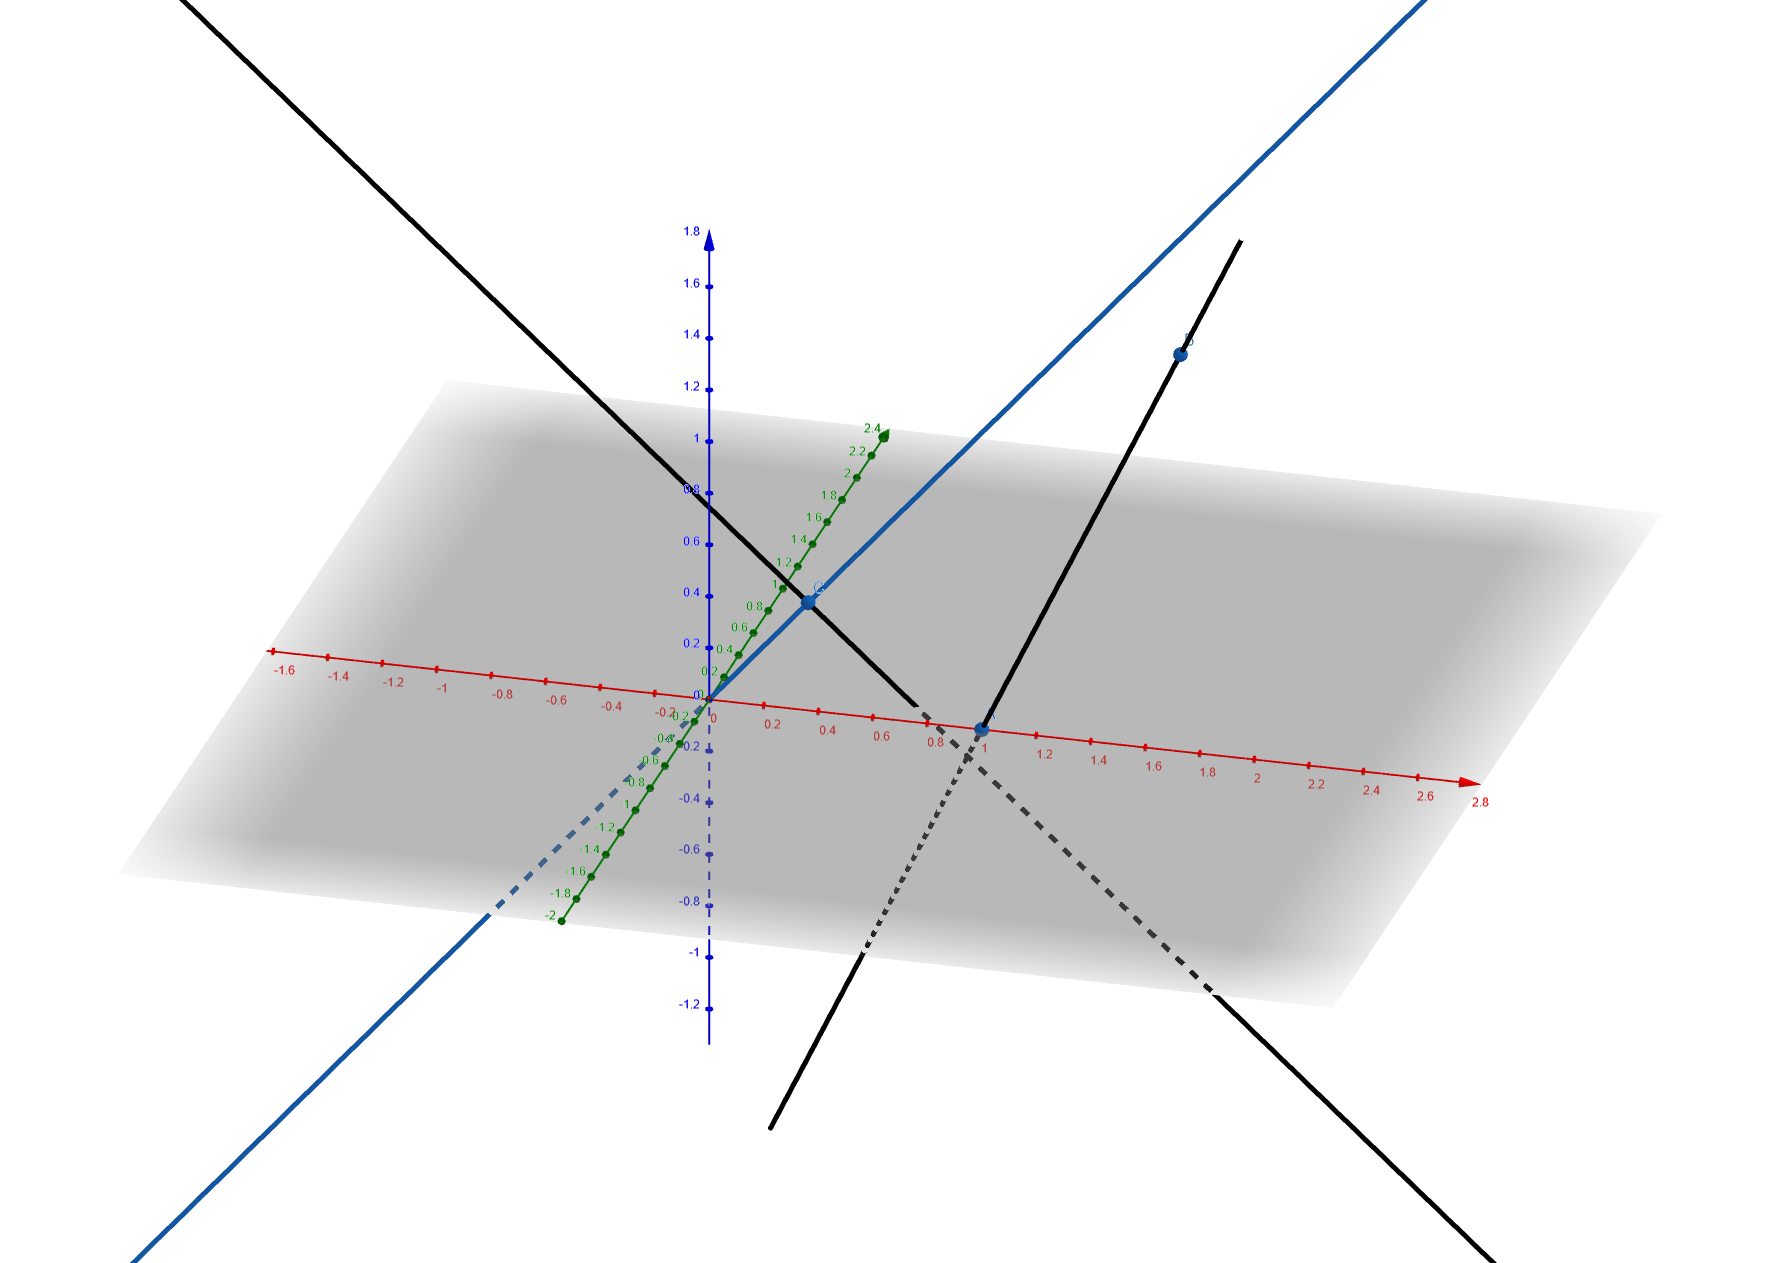
\includegraphics[width=\paperwidth]{resources/1.5_figure.png}
        \caption{Чертёж}
        \label{fig:main_figure}
    \end{sidewaysfigure}
    \FloatBarrier


\end{document}